\lecture{Lecture - 11\hfill 16 Oct 24}

\begin{proof}
	We prove this by induction on $l.$ For $l=1,$ the theorem holds 
	true because the only walks of length $1,$ from a vertex $x$ to 
	a vertex $y$ are the edges from $x$ to $y.$  So the number of
	walks of length $1$ from $x$ to $y$ is exactly the number of
	edges from $x$ to $y.$ Now suppose the theorem holds for $i=
	1, \dotsc, k-1.$ Suppose $x,$ $y$ in $V$ are arbitrarily given.
	We will prove that the number of walks from $x$ to $y$ of length
	$k$ is $A^k(x,y).$ Let $x = v_0, e_1, v_1, \dotsc, e_{k-1},
	v_{k-1}, e_k, v_k = y$ denote a walk $w$ from $x$ to $y$ of 
	length $k.$ So, each walk of length $l$ from $x$ to $y$ is
	a concatenation of a some $w'$ in $W_{k-1}(x,v_{k-1})$ and 
	some edge from $v_{k-1}$ to $y$ where $v_{k-1}$ is some vertex 
	in $V$ and $W_{k-1}(x, v)$ denotes the number of walks of length
	$k-1$ from a vertex $x$ to a vertex $v$ in $V.$
	Conversely, if $w'$ is in $W_{k-1}(x,v)$ and $e$ is an edge from
	$v$ to $y$ for some vertex $v$ in $V,$ then the concatenation
	$w' \ast e$ is a walk of length $k$ from $x$ to $y.$
	Using the induction hypothesis, we have $ \lvert W_{k-1}(x,v) \rvert = A^{k-1} (x,v)$ for all $x$ and $v$ in $V.$
	So, we have the cardinality of $W_{k}(x,y) = 
	\sum_{v\in V} \lvert W_{k-1}(x,v) \rvert A(v,y) = 
	(A^{k-1} A)(x,y) = A^k (x,y).$
\end{proof}

\begin{corollary}[]
	Let $G = (V,E)$ be a simple graph with $\lvert V \rvert = n,$
	adjacency matrix $A,$ and $\lambda_1 \geq \lambda _2 \geq \cdots
	\geq \lambda_n$ are the characteristic values of $A,$ then the
	number of closed walks of length $l$ in $G$ is
	$\lambda_l^1 + \lambda_2^2 + \cdots \lambda_n^l.$
\end{corollary}


\begin{figure}[h]
\centering
	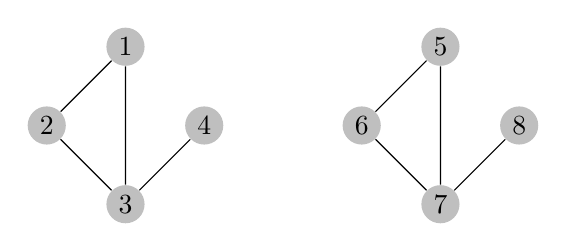
\begin{tikzpicture}
		\tikzstyle{vertex}=[circle,fill=black!25,minimum size=12pt,inner sep=2pt]
		\node[vertex] (g_1) at (2,2) {1};
		\node[vertex] (g_2) at (1,1) {2};
		\node[vertex] (g_3) at (2,0) {3};
		\node[vertex] (g_4) at (3,1) {4};
		\node[vertex] (g_5) at (6,2) {5};
		\node[vertex] (g_6) at (5,1) {6};
		\node[vertex] (g_7) at (6,0) {7};
		\node[vertex] (g_8) at (7,1) {8};
		\draw (g_1) -- (g_2) -- (g_3) --(g_1);
		\draw (g_3) -- (g_4);
		\draw (g_5) -- (g_6) -- (g_7) -- (g_5);
		\draw (g_7) -- (g_8);
	\end{tikzpicture}
\end{figure}


The two graphs above have different labels but the same structure.

\begin{definition}[Isomorphism]
	An isomorphism between graphs $G_1 = (V_1, E_1)$ and $G_2 = 
	(V_2, E_2)$ is a bijection $\sigma \colon V_1 \to V_2.$
	such that $\{ i,j \} $ is in $E_1$ if and only if
	$\{ \sigma(i), \sigma(j) \}$ is in $E_2.$
\end{definition}

\begin{remark}
	The permutation $\sigma$ relabels the vertices of $G_1$
	but does not change its structure.
\end{remark}

\begin{figure}[h]
	\centering
\tikz[rotate = 90]\graph{
	{1,2,3} -- [complete bipartite] {4,5,6};
};
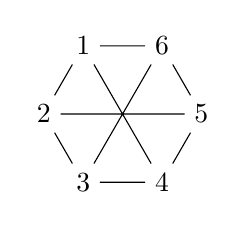
\begin{tikzpicture}
	\foreach \i in {0,1,2,3,4,5}{
		\node (g\i) at (60*\i+120:1) {\number\numexpr \i + 1\relax};
	}
	
	\draw (g1)--(g2)--(g3)--(g4)--(g5)--(g0)--(g1);
	\draw (g1)--(g4) (g2)--(g5) (g3)--(g0);
\end{tikzpicture}
\end{figure}

\begin{theorem}
	Let $G_1,$ $G_2$ are graphs on a vertex set $V,$ then
	$G_1 \equiv G_2$ if and only if there exists a permutation
	matrix $P$ such that $A_1 = P^{-1} A_2 P$
	where $A_1, $ respectively $A_2$ are the adjacency matrices 
	of $G_1,$ respectively $G_2.$
\end{theorem}

A permutation matrix is any matrix which has exactly one nonzero entry
in each row or column and consists of only $0$s and $1$.
So, there is a bijective correspondence between permutations $\sigma$
in $S_n$ and permutation matrices of size $n \times  n$ given by
$\sigma \leftrightarrow P_\sigma$
where 
$$ P_\sigma(i,j) = \begin{cases}
1 & \text{ if } i = \sigma(j) \\
0 & \text{ otherwise } \\
\end{cases}.$$
Also, $P_\sigma P_\tau = P_{\sigma \tau}$ and $P_\sigma^{-1}=  
P_{\sigma^{-1}}.$

